\documentclass{article}
\usepackage[top = 1.5cm, bottom = 1.5cm, left = 2cm, right = 2cm]{geometry}
\usepackage{lmodern}
\usepackage[czech]{babel}

\usepackage{amsmath}
\usepackage{amssymb}
\usepackage{bbm}
\usepackage{mathtools}
\usepackage{nicefrac}


\def\R{\mathbb{R}}
\def\C{\mathbb{C}}
\def\D{\mathcal{D}}
\def\Cont{\mathcal{C}}
\def\supp{\operatorname{supp}}
\def\L{\mathcal{L}}
\def\Res{\operatorname{Res}}

\newcommand{\e}[1]{\mathrm{e}^{\textstyle #1}}
\def\i{\mathrm{i}}

\begin{document}

\section*{MpF 3: Domácí úkol 1}
\textbf{Autor: Michal Grňo}

\subsection*{Příklad č. 1}
\subsubsection*{Zadání}
Dokažte konvergenci dvou posloupností v $\D'(\R)$ se slabou$^*$ topologií:
\begin{gather*}
    n \, \big( \delta_{\nicefrac{1}{n}} - \delta_0 \big)
    \quad \longrightarrow \quad
    -\delta_0 '
    \\[5pt]
    n^2 \, \big(
        \delta_{-\nicefrac{1}{n}}
        -2 \, \delta_0
        + \delta_{\nicefrac{1}{n}}
    \big)
    \quad \longrightarrow \quad
    \text{?}
\end{gather*}

\subsubsection*{Řešení}
Začneme první posloupností:
\begin{align*}
    n \, \big( \delta_{\nicefrac{1}{n}} - \delta_0 \big)
    \quad &\longrightarrow \quad
    -\delta_0 '
    \\[3pt]
    &\Updownarrow
    \\[3pt]
    \Big< n \, \big( \delta_{\nicefrac{1}{n}} - \delta_0 \big), \; \varphi \Big>
    \quad &\longrightarrow \quad
    \Big< -\delta_0 ', \; \varphi \Big>
    \quad \forall \varphi \in \D(\R)
    \\[3pt]
    &\Updownarrow
    \\[3pt]
    n \, \big( \varphi(\nicefrac{1}{n}) - \varphi(0) \big)
    \quad &\longrightarrow \quad
    \varphi'(0)
    \qquad \forall \varphi \in \D(\R)
    \\[3pt]
    &\Updownarrow
    \\[3pt]
    \lim_{n \to \infty} \frac{ \varphi(\nicefrac{1}{n}) - \varphi(0) }{\nicefrac{1}{n}}
    &= \varphi'(0)
    \qquad \forall \varphi \in \D(\R)
    \\[3pt]
    &\Uparrow
    \\[3pt]
    \lim_{t \to 0} \frac{ \varphi(t) - \varphi(0) }{t}
    &= \varphi'(0)
    \qquad \forall \varphi \in \D(\R)
\end{align*}
Poslední řádek ale není nic jiného než definice derivace, rovnost tedy platí a máme dokázanou konvergenci.

\bigskip

Pokračujeme druhou posloupností:
\begin{equation*}
    g_n =
    n^2 \, \big(
        \delta_{-\nicefrac{1}{n}}
        -2 \, \delta_0
        + \delta_{\nicefrac{1}{n}}
    \big)
\end{equation*}
Nejprve se omezíme pouze na testovací funkce analytické na $[-1, 1]$:
\begin{align*}
    \varphi &\in M \coloneqq \D( \R ) \cap \Cont^\omega([-1,1])
    &
    \varphi(x) &= \sum_{k=0}^\infty \alpha_k \, x^k,
    \quad x \in [-1, 1]
\end{align*}
Taylorova řada $\varphi$ konverguje dokonce stejnoměrně vůči $x$ – to nám později umožní prohazovat limity pro $n$ a $k$.
\begin{align*}
    \Big< g_n, \; \varphi \Big>
    &= n^2 \, \big(
        \varphi(-\nicefrac{1}{n})
        -2 \, \varphi(0)
        + \varphi(\nicefrac{1}{n})
    \big)
    \\[5pt]
    &= n^2 \, \Bigg(
        \sum_{k=0}^\infty a_k \, \big( -\nicefrac{1}{n} \big)^k
        - 2 \, a_0
        + \sum_{k=0}^\infty a_k \, \big( \nicefrac{1}{n} \big)^k
    \Bigg)
    \\[5pt]
    &= n^2 \, \Bigg(
        \sum_{k=1}^\infty a_k \, \big( -\nicefrac{1}{n} \big)^k
        + \sum_{k=1}^\infty a_k \, \big( \nicefrac{1}{n} \big)^k
    \Bigg)
    \\[5pt]
    &= n^2 \, \sum_{k=1}^\infty
    \frac{(-1)^k \, a_k + a_k}{n^k}
    \\[5pt]
    &= 2 \, a_2
    + \frac{2 \, a_4}{n^2}
    + \frac{2 \, a_6}{n^4}
    + \frac{2 \, a_8}{n^6}
    + \, ...
    \;\stackrel{n}{\longrightarrow}\;
    2 \, a_2 = \varphi''(0) = \Big< \delta_0'', \; \varphi \Big>
\end{align*}
Dokázali jsme tedy, že restrikce $g_n$ na $M$ konverguje k distribuci $\delta_0''$. Nyní bychom chtěli ukázat, že $M$ je hustá v $\D(\R)$ a využít spojitosti distribucí, abychom tuto konvergenci ukázali i pro neanalytické funkce.

\bigskip

Vyjdeme z toho, že $\Cont^\omega([-1,1])$ je hustá v $\Cont^\infty([-1,1])$ (Nachbinův teorém). Dovolíme-li funkcím z $\Cont^\infty([-1,1])$ libovolná hladká rozšíření na $\R$ taková, že mají kompaktní nosič, dostáváme přesně $\D(\R)$. Dovolíme-li totéž funkcím z $\Cont^\omega([-1,1])$, dostaneme zákonitě množinu hustou v $\D(\R)$. Proto můžeme pro každou funkci $\varphi \in \D(\R)$ najít posloupnost $\{\varphi_k\} \subset M$, že $\varphi_k \rightrightarrows \varphi$. Máme tedy:
\begin{align*}
    \Big< g_n, &\; \varphi_k \Big>
    \quad \stackrel{k}{\rightrightarrows} \quad
    \Big< g_n, \; \varphi \Big>
    \\
    &\big\downarrow {}^n
    \\
    \Big<\delta_0'', &\; \varphi_k \Big>
    \quad \stackrel{k}{\rightrightarrows} \quad
    \Big< \delta_0'', \; \varphi \Big>
\end{align*}
„Dokreslit poslední šipku“ nám umožňuje Moorův-Osgoodův teorém. Dokázali jsme tedy, že
\begin{equation*}
    \Big<g_n, \; \varphi \Big>
    \quad \longrightarrow \quad
    \Big<\delta_0'', \; \varphi \Big>
    \qquad
    \forall \varphi \in \D(\R)
\end{equation*}

\subsubsection*{Závěr}
Dokázali jsme, že:
\begin{gather*}
    n \, \big( \delta_{\nicefrac{1}{n}} - \delta_0 \big)
    \quad \longrightarrow \quad
    -\delta_0 '
    \\[5pt]
    n^2 \, \big(
        \delta_{-\nicefrac{1}{n}}
        -2 \, \delta_0
        + \delta_{\nicefrac{1}{n}}
    \big)
    \quad \longrightarrow \quad
    \delta_0''
\end{gather*}

\pagebreak

\subsection*{Příklad č. 2}
\subsubsection*{Zadání}
Máme RLC obvod:
\begin{figure}[h!]
    \centering
    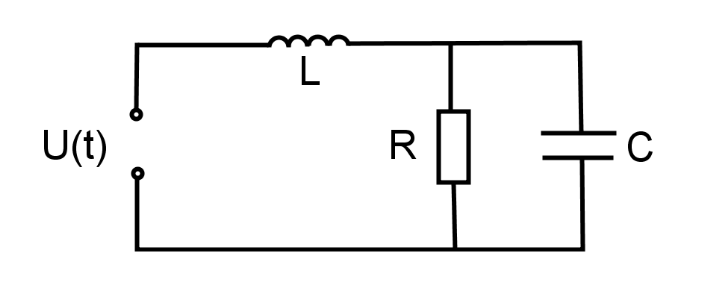
\includegraphics[width=5cm]{rlc.png}
\end{figure}

\vspace{2em}

\noindent
Pro napětí na zdroji platí
\begin{equation*}
    U(t) = U_0 \; \theta(t) \; \e{\i \omega t} \: ,
\end{equation*}
kde $\theta(t)$ je Heavisidova funkce. Je splněna podmínka $L > 4 \, R^2 C$. Nalezněte ustálený proud $I_{\rm u}(t)$.

\subsubsection*{Řešení}
Úlohu budeme řešit pomocí Laplaceovy transformace. Nejprve vypočítáme transformované vstupní napětí:
\begin{equation*}
    u(p) = \L( \, t \mapsto U(t) \, )(p) = \frac{U_0}{p - \i \omega}
\end{equation*}
Následně podle obrázku vyjádříme komplexní impedanci obvodu:
\begin{equation*}
    z(p) = L \, p + \left( \frac{1}{R} + C \, p \right)^{\!-1}
    = \frac{R + L\,p + RLC \, p^2}{1 + RC \, p}
\end{equation*}
Z transformované verze Ohmova zákona $u(p) = z(p) \, i(p)$ potom plyne:
\begin{align*}
    i(p) = \frac{\, u(p) \,}{z(p)}
    = \frac{U_0}{p - \i \omega} \;
    \frac{1 + RC \, p}{R + L\,p + RLC \, p^2}
\end{align*}
Chceme provést zpětnou Laplaceovu transformaci $i(p) \mapsto I(t)$ pomocí reziduové věty a $i(p)$ je racionální funkce, proto faktorizujeme jmenovatel:
\begin{equation*}
    (p - \i\omega)(R + L \, p + RLC \, p^2)
    = (p - a)(p - b)(p - c)
\end{equation*}
\begin{align*}
    a &= \i\omega \\[8pt]
    b &= -\frac{1}{2RC} + \sqrt{\frac{1}{4 R^2 C^2} - \frac{1}{LC}} \\[8pt]
    c &= -\frac{1}{2RC} - \sqrt{\frac{1}{4 R^2 C^2} - \frac{1}{LC}}
\end{align*}
Fyzikálně požadujeme, aby $R,L,C$ byla kladná reálná čísla. Ze zadání navíc víme, že $L > 4 R^2 C$, tedy $LC > 4 R^2 C^2$. Proto budou kořeny $b,c$ reálné a záporné. Pro zpětnou Laplaceovu transformaci platí:
\begin{equation*}
    I(t) \;=\; \L^{-1}(\, p \mapsto i(p) \,)(t) \;=\;
    \e{at} \; \Res_a i(p) \;+\; \e{bt} \; \Res_b i(p) \;+\; \e{ct} \; \Res_c i(p)
\end{equation*}
Nás ovšem zajímá pouze ustálený proud – členy $\e{\scriptstyle bt}$ a $\e{\scriptstyle ct}$ půjdou v $t\to\infty$ do nuly, proto pro ustálený proud dostáváme vztah:
\begin{equation*}
    I_{\rm u}(t) \;=\;
    \e{at} \; \Res_a i(p) \;=\;
    U_0 \; \e{\i\omega t} \;
    \frac{1 + \i \omega RC}{R + \i \omega L - \omega^2 RLC}
    \: .
\end{equation*}


\end{document}
